% -----------------------------------------------------------------------------
% Conteudo AODV-EN. Template base: Prof. Wesley Pacheco Calixto (IFG).
% -----------------------------------------------------------------------------
\chapter{PROJETO E IMPLEMENTAÇÃO DO ALGORITMO
AODV-EN}\label{projeto-e-implementauxe7uxe3o-do-algoritmo-aodv-en}

Este capítulo apresenta o projeto e a implementação do algoritmo
AODV-EN, desenvolvido como uma adaptação do protocolo AODV para redes
mesh baseadas em ESP-NOW. A apresentação foi organizada de forma
progressiva, partindo da visão geral da arquitetura até os mecanismos
internos de descoberta de rotas, encaminhamento de dados, manutenção de
rotas e tratamento de falhas. Ao final, são discutidas as principais
adaptações realizadas em relação ao AODV original, considerando as
restrições específicas do ESP-NOW. \#\# Visão Geral da Arquitetura do
AODV-EN A arquitetura do AODV-EN foi concebida em camadas, de modo a
separar as responsabilidades entre aplicação, interface pública de
integração, núcleo do protocolo, adaptador de transporte e meio de
comunicação ESP-NOW. Essa separação reduz o acoplamento entre os
componentes, favorece a manutenção do código e permite a evolução
incremental do artefato sem comprometer o funcionamento global da
solução. A Figura 3 apresenta a organização geral da arquitetura
proposta, evidenciando o fluxo de interação entre as camadas
responsáveis pela aplicação, pela interface pública da pilha, pelo
núcleo do protocolo, pelo adaptador de transporte e pelo meio de
comunicação ESP-NOW.
\begin{figure}[H]
\centering
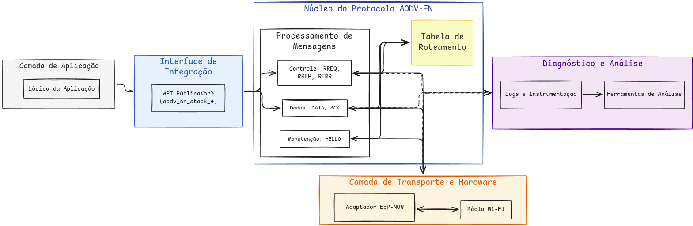
\includegraphics[width=0.85\textwidth,keepaspectratio]{figuras/image3.png}
\caption{Figura 3 -- Arquitetura geral do AODV-EN}
\end{figure}
A camada de aplicação é responsável por acionar o envio de dados e
registrar eventos de execução. A interface pública disponibiliza as
funções de inicialização, envio, recepção e atualização temporal da
pilha. O núcleo do protocolo concentra a lógica de roteamento, incluindo
descoberta de rotas, manutenção de tabelas, tratamento de falhas e
encaminhamento de pacotes. O adaptador ESP-NOW, por sua vez, encapsula
os detalhes de transmissão e recepção na camada de enlace.

\section{Estrutura Modular da
Implementação}\label{estrutura-modular-da-implementauxe7uxe3o}

A implementação do AODV-EN foi organizada em módulos funcionais com
interfaces explícitas, buscando separar a lógica central do protocolo
das estruturas auxiliares e dos detalhes específicos do transporte. Essa
organização contribui para a manutenção do código, facilita a validação
isolada de componentes e permite maior rastreabilidade entre as decisões
de projeto e sua materialização no firmware. A interface pública da
pilha é concentrada nos módulos aodv\_en.h e aodv\_en.c, responsáveis
por expor funções de inicialização, envio, recepção, atualização
temporal e consulta de estatísticas. O núcleo do protocolo é
implementado principalmente no módulo aodv\_en\_node.c, que coordena os
processos de descoberta de rotas, encaminhamento de dados, manutenção de
estados e tratamento de mensagens. Os demais módulos implementam
estruturas de apoio, como tabela de rotas, tabela de vizinhos, cache de
RREQ, gerenciamento de peers e manipulação de endereços MAC. A Figura 4
apresenta a organização modular da implementação, evidenciando a relação
entre a aplicação, a fachada pública da pilha, o núcleo do protocolo, os
módulos auxiliares e o adaptador ESP-NOW.
\begin{figure}[H]
\centering
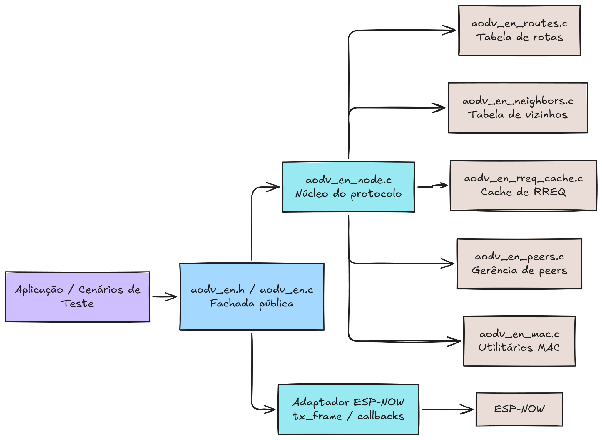
\includegraphics[width=0.85\textwidth,keepaspectratio]{figuras/image4.png}
\caption{Figura 4 -- Estrutura modular da implementação do AODV-EN}
\end{figure}

\section{Estruturas de Dados
Utilizadas}\label{estruturas-de-dados-utilizadas}

As estruturas de dados do AODV-EN foram projetadas considerando as
limitações de memória do ambiente embarcado e a necessidade de
atualização em tempo real das informações de roteamento. Essas
estruturas armazenam o estado local de cada nó e permitem a execução dos
mecanismos de descoberta, seleção, manutenção e invalidação de rotas. O
Quadro 12 apresenta uma síntese das principais estruturas utilizadas na
implementação do AODV-EN e sua função no funcionamento do protocolo.
\textbf{Quadro 12 -- Estruturas de dados utilizadas no AODV-EN}

{\def\LTcaptype{none} % do not increment counter
\begin{longtable}[]{@{}
  >{\raggedright\arraybackslash}p{(\linewidth - 4\tabcolsep) * \real{0.3333}}
  >{\raggedright\arraybackslash}p{(\linewidth - 4\tabcolsep) * \real{0.3333}}
  >{\raggedright\arraybackslash}p{(\linewidth - 4\tabcolsep) * \real{0.3333}}@{}}
\toprule\noalign{}
\begin{minipage}[b]{\linewidth}\raggedright
Estrutura
\end{minipage} & \begin{minipage}[b]{\linewidth}\raggedright
Função principal
\end{minipage} & \begin{minipage}[b]{\linewidth}\raggedright
Papel no protocolo
\end{minipage} \\
\midrule\noalign{}
\endhead
\bottomrule\noalign{}
\endlastfoot
Tabela de rotas & Armazenar destinos conhecidos, próximo salto, estado,
métrica e expiração & Permite seleção e encaminhamento de pacotes por
rotas válidas \\
Tabela de vizinhos & Registrar nós alcançáveis diretamente e informações
de RSSI & Subsidia o cálculo da métrica híbrida e a manutenção da
conectividade local \\
Cache de RREQ & Armazenar requisições de rota já processadas & Evita
duplicatas, retransmissões desnecessárias e ciclos de propagação \\
Gerenciamento de peers & Controlar pares registrados no ESP-NOW &
Permite operar dentro das limitações de peers simultâneos do ESP-NOW \\
\end{longtable}
}

\textbf{Fonte: Elaborado pelos autores.}

\subsection{Tabela de Rotas}\label{tabela-de-rotas}

\begin{verbatim}
A tabela de rotas mantém, para cada destino conhecido, informações como próximo salto, número de saltos, número de sequência, estado da rota, métrica de custo e tempo de expiração. Essa estrutura é essencial para o encaminhamento de pacotes, pois permite identificar se existe uma rota válida para determinado destino e qual vizinho deve ser utilizado como próximo salto.
\end{verbatim}

A atualização das entradas considera critérios de frescor da informação,
qualidade da rota e validade temporal, preservando o princípio do AODV
de priorizar rotas mais recentes e evitar informações obsoletas. Além
disso, a implementação emprega critérios de substituição que consideram
número de sequência, métrica, contagem de saltos e tempo de expiração,
reduzindo trocas instáveis de rota e contribuindo para maior
estabilidade do protocolo.

\subsection{Tabela de Vizinhos}\label{tabela-de-vizinhos}

A tabela de vizinhos registra os nós alcançáveis diretamente por um
determinado nó da rede. Para cada vizinho, são armazenadas informações
como endereço MAC, estado do enlace, último RSSI observado, RSSI médio,
instante da última comunicação e eventos de falha de enlace.

Essa estrutura subsidia tanto o encaminhamento local quanto o cálculo da
métrica híbrida de roteamento. Ao considerar informações de RSSI, o
AODV-EN pode avaliar não apenas a quantidade de saltos até o destino,
mas também a qualidade dos enlaces utilizados no caminho, favorecendo
rotas potencialmente mais estáveis em ambientes sem fio sujeitos a
interferências e variações de sinal.

\subsection{Cache de RREQ}\label{cache-de-rreq}

O cache de RREQ armazena pares formados pelo endereço do nó originador e
pelo identificador da requisição de rota. Esse mecanismo permite
reconhecer requisições já processadas, evitando que uma mesma mensagem
RREQ seja tratada repetidamente por um nó.

A utilização desse cache é fundamental em processos de flooding
controlado, pois reduz retransmissões redundantes, limita a propagação
excessiva de mensagens de controle e contribui para prevenir ciclos
durante a descoberta de rotas. Dessa forma, o cache de RREQ atua como
mecanismo de controle de overhead e de estabilidade do processo de
descoberta.

\subsection{Gerenciamento de Peers}\label{gerenciamento-de-peers}

O gerenciamento de peers foi projetado para lidar com a limitação de
pares simultâneos imposta pelo ESP-NOW. Como o protocolo exige que
dispositivos sejam registrados como peers para comunicação unicast, essa
restrição pode limitar a escalabilidade da rede quando há múltiplos nós
participantes.

Para contornar essa limitação, o AODV-EN separa a vizinhança lógica
mantida pelo protocolo da tabela física de peers utilizada pelo ESP-NOW.
Quando necessário, aplica-se uma política LRU (Least Recently Used),
substituindo pares menos recentemente utilizados e permitindo que o
protocolo opere com um número de nós maior que o limite simultâneo de
peers registrados. Essa estratégia preserva a compatibilidade com o
ESP-NOW sem comprometer a dinâmica de descoberta e manutenção de rotas.

\section{Mensagens do Protocolo}\label{mensagens-do-protocolo}

O AODV-EN utiliza mensagens de controle e de dados para realizar a
descoberta, manutenção e utilização das rotas na rede. As mensagens de
controle são responsáveis por estabelecer caminhos, atualizar estados,
manter a conectividade local e tratar falhas de enlace. Já as mensagens
de dados transportam a carga útil da aplicação entre origem e destino,
utilizando as rotas previamente descobertas pelo protocolo. A definição
dessas mensagens foi baseada nos princípios do AODV, especialmente
quanto ao uso de requisições de rota, respostas de rota e mensagens de
erro. Entretanto, foram incorporadas adaptações necessárias ao contexto
do ESP-NOW, como o uso de endereçamento por MAC, limitação de tamanho de
payload, controle de TTL e suporte à confirmação em nível de aplicação.
O Quadro 13 apresenta uma síntese das mensagens utilizadas pelo AODV-EN
e suas respectivas funções no protocolo. \textbf{Quadro 13 -- Mensagens
utilizadas pelo AODV-EN}

{\def\LTcaptype{none} % do not increment counter
\begin{longtable}[]{@{}
  >{\raggedright\arraybackslash}p{(\linewidth - 6\tabcolsep) * \real{0.2500}}
  >{\raggedright\arraybackslash}p{(\linewidth - 6\tabcolsep) * \real{0.2500}}
  >{\raggedright\arraybackslash}p{(\linewidth - 6\tabcolsep) * \real{0.2500}}
  >{\raggedright\arraybackslash}p{(\linewidth - 6\tabcolsep) * \real{0.2500}}@{}}
\toprule\noalign{}
\begin{minipage}[b]{\linewidth}\raggedright
Mensagem
\end{minipage} & \begin{minipage}[b]{\linewidth}\raggedright
Tipo
\end{minipage} & \begin{minipage}[b]{\linewidth}\raggedright
Função principal
\end{minipage} & \begin{minipage}[b]{\linewidth}\raggedright
Uso no protocolo
\end{minipage} \\
\midrule\noalign{}
\endhead
\bottomrule\noalign{}
\endlastfoot
RREQ & Controle & Requisitar descoberta de rota & Emitida quando um nó
precisa alcançar um destino para o qual não possui rota válida \\
RREP & Controle & Responder a uma requisição de rota & Retorna pelo
caminho reverso para estabelecer ou atualizar a rota até o destino \\
RERR & Controle & Notificar erro ou quebra de rota & Informa falhas de
enlace e permite invalidar rotas afetadas \\
HELLO & Controle & Manter vizinhança local & Atualiza a conectividade
entre nós diretamente alcançáveis \\
DATA & Dados & Transportar a carga útil da aplicação & Encaminhada salto
a salto conforme a tabela de rotas \\
ACK & Controle/aplicação & Confirmar recebimento de dados & Apoia a
verificação de entrega e o cálculo de métricas de confiabilidade \\
\end{longtable}
}

\textbf{Fonte: Elaborado pelos autores.}

As mensagens RREQ, RREP e RERR compõem o núcleo do mecanismo de
roteamento reativo do AODV-EN. A mensagem RREQ é utilizada quando a
origem necessita descobrir uma rota para determinado destino. Ao ser
propagada pela rede, ela permite que os nós intermediários estabeleçam
rotas reversas para a origem. A mensagem RREP, por sua vez, retorna pelo
caminho reverso e permite a formação da rota direta até o destino. Já a
mensagem RERR é utilizada quando ocorre falha de enlace ou invalidação
de rota, permitindo que os nós afetados atualizem suas tabelas e iniciem
nova descoberta, se necessário.

A mensagem HELLO é utilizada para manutenção da vizinhança local,
permitindo identificar nós diretamente alcançáveis e atualizar
informações associadas aos enlaces. Essas informações são importantes
para a manutenção das rotas e para o cálculo da métrica híbrida baseada
em número de saltos e qualidade do sinal.

As mensagens DATA e ACK estão associadas à comunicação da aplicação. A
mensagem DATA transporta a carga útil entre origem e destino, utilizando
as rotas válidas mantidas pelo protocolo. Quando necessário, a mensagem
ACK confirma o recebimento dos dados em nível de aplicação, contribuindo
para a avaliação da confiabilidade da entrega e para o controle de
retransmissões.

\section{Funcionamento do Algoritmo}\label{funcionamento-do-algoritmo}

O funcionamento do AODV-EN pode ser compreendido a partir de quatro
processos principais: descoberta de rotas, encaminhamento de dados,
manutenção de rotas e tratamento de falhas. Esses processos operam de
forma integrada para permitir a comunicação multi-hop em redes baseadas
em ESP-NOW, preservando a característica reativa do protocolo AODV
original. De modo geral, quando um nó precisa enviar dados para um
destino e não possui rota válida, o protocolo inicia um processo de
descoberta de rota. Após a definição do caminho, os pacotes de dados são
encaminhados de salto a salto até o destino. Durante a operação da rede,
mecanismos de manutenção verificam a validade das rotas e a
conectividade entre vizinhos. Caso ocorra falha de enlace, as rotas
afetadas são invalidadas e uma nova descoberta pode ser iniciada. \#\#\#
Descoberta de Rotas A descoberta de rotas é iniciada quando um nó de
origem precisa enviar dados para um destino e não possui uma rota válida
em sua tabela de roteamento. Nessa situação, o nó originador emite uma
mensagem RREQ contendo informações como endereço de origem, endereço de
destino, identificador da requisição, número de sequência e limite de
propagação. Ao receber uma mensagem RREQ, cada nó intermediário verifica
se a requisição já foi processada anteriormente. Caso seja uma
requisição duplicada, ela é descartada. Caso contrário, o nó registra ou
atualiza uma rota reversa para a origem, incrementa o contador de saltos
e retransmite a requisição conforme a política de disseminação
configurada. Quando a mensagem RREQ alcança o destino, ou um nó que
possua rota válida para ele, é gerada uma mensagem RREP. Essa resposta
retorna em unicast pelo caminho reverso previamente estabelecido,
permitindo que os nós intermediários atualizem suas rotas diretas até o
destino. Ao receber o RREP, a origem passa a possuir uma rota válida e
pode iniciar o envio dos dados pendentes. A Figura 5 apresenta o fluxo
de descoberta de rotas no AODV-EN, destacando a propagação da mensagem
RREQ e o retorno da mensagem RREP pelo caminho reverso.
\begin{figure}[H]
\centering
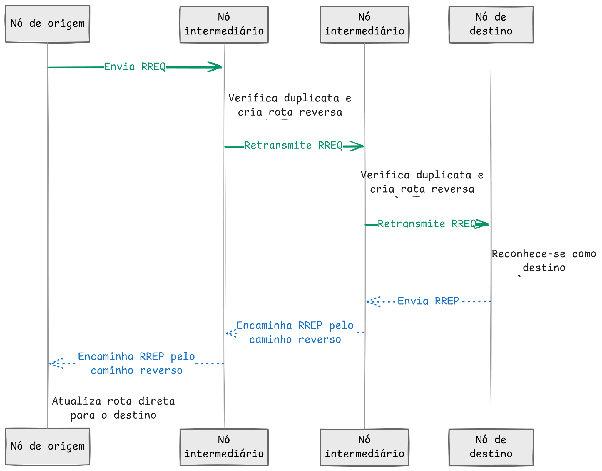
\includegraphics[width=0.85\textwidth,keepaspectratio]{figuras/image5.png}
\caption{Figura 5 -- Fluxo de descoberta de rotas no AODV-EN}
\end{figure}
\#\#\# Encaminhamento de Dados Após a descoberta de uma rota válida, o
encaminhamento dos dados ocorre de forma salto a salto. O nó de origem
consulta sua tabela de rotas para identificar o próximo salto em direção
ao destino e transmite a mensagem DATA ao vizinho correspondente. Cada
nó intermediário repete o mesmo procedimento, consultando sua própria
tabela de rotas até que o pacote alcance o destino final. Caso a origem
não possua rota válida no momento da tentativa de envio, o pacote é
armazenado temporariamente em uma fila de dados pendentes. Em seguida, o
protocolo inicia o processo de descoberta de rota por meio do envio de
uma mensagem RREQ. Quando a rota é estabelecida, os dados pendentes são
transmitidos conforme o caminho descoberto. Esse mecanismo permite que a
aplicação solicite o envio de dados mesmo quando a rota ainda não está
disponível, preservando a característica reativa do AODV-EN e evitando o
descarte imediato de pacotes em situações de descoberta inicial.

\subsection{Manutenção de Rotas}\label{manutenuxe7uxe3o-de-rotas}

A manutenção de rotas tem como objetivo preservar a validade das
informações de roteamento durante a operação da rede. Para isso, o
AODV-EN utiliza mecanismos de controle baseados em mensagens periódicas,
temporizadores de expiração e atualização do estado dos vizinhos. As
mensagens HELLO são utilizadas para manter a conectividade local entre
nós diretamente alcançáveis. A partir dessas mensagens, cada nó atualiza
sua tabela de vizinhos, registrando informações como instante da última
comunicação, estado do enlace e intensidade do sinal recebido. Essas
informações contribuem para identificar vizinhos ativos e subsidiar o
cálculo da métrica híbrida de roteamento. Além da manutenção da
vizinhança, cada rota possui um tempo de validade associado. Rotas que
permanecem sem uso ou ultrapassam seu tempo de expiração deixam de ser
consideradas válidas para encaminhamento. Esse mecanismo reduz o uso de
informações obsoletas e contribui para evitar encaminhamentos por
caminhos indisponíveis. A manutenção de rotas também está relacionada ao
controle de estabilidade. Ao atualizar uma rota existente, o protocolo
considera critérios como número de sequência, métrica, contagem de
saltos e tempo de expiração, evitando substituições frequentes quando a
nova rota não apresenta melhoria significativa. \#\#\# Tratamento de
Falhas O tratamento de falhas é acionado quando o protocolo identifica
indisponibilidade de um enlace ou impossibilidade de encaminhar dados
por uma rota previamente considerada válida. Essa detecção pode ocorrer
por ausência de resposta, falha de transmissão, expiração de vizinhança
ou perda de conectividade com o próximo salto. Ao detectar uma falha, o
nó invalida as rotas que dependem do enlace afetado e gera uma mensagem
RERR para notificar os nós impactados. Essa mensagem permite que os
demais nós atualizem suas tabelas de roteamento, evitando o uso de
caminhos inválidos. Quando ainda existem dados pendentes para o destino
afetado, o protocolo pode iniciar uma nova descoberta de rota por meio
de RREQ. Esse mecanismo permite que o AODV-EN reaja dinamicamente a
alterações na topologia da rede, buscando restabelecer a comunicação por
rotas alternativas quando disponíveis. Dessa forma, o tratamento de
falhas contribui para a capacidade de auto-recuperação da rede mesh. A
Figura 6 apresenta o fluxo de tratamento de falhas e reconvergência do
AODV-EN, desde a detecção da falha até a tentativa de restabelecimento
da comunicação.
\begin{figure}[H]
\centering
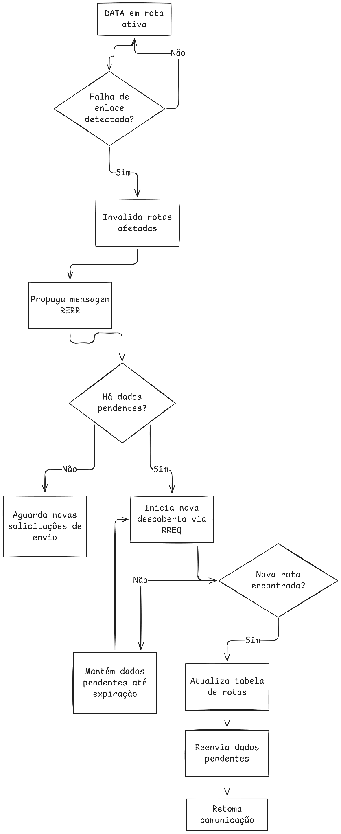
\includegraphics[width=0.85\textwidth,keepaspectratio]{figuras/image6.png}
\caption{Figura 6 -- Fluxo de tratamento de falhas e reconvergência no AODV-EN}
\end{figure}
\#\# Adaptações do AODV para ESP-NOW A adaptação do AODV para operação
sobre ESP-NOW exigiu modificações relacionadas ao endereçamento, à
disseminação de mensagens, ao gerenciamento de peers e à métrica de
seleção de rotas. Essas adaptações foram necessárias porque o ESP-NOW
opera na camada de enlace, utiliza endereçamento baseado em MAC, possui
limitação no número de peers registrados simultaneamente e não oferece,
de forma nativa, mecanismos completos para roteamento multi-hop. Dessa
forma, o AODV-EN preserva os princípios fundamentais do AODV, como
descoberta de rotas sob demanda, uso de mensagens de controle,
manutenção de tabelas de roteamento e tratamento de falhas, mas
incorpora mecanismos específicos para viabilizar sua execução em
dispositivos ESP32 utilizando ESP-NOW. O Quadro 14 sintetiza as
principais adaptações realizadas no AODV-EN em relação ao AODV original.
\textbf{Quadro 14 -- Principais adaptações do AODV para o contexto do
ESP-NOW}

{\def\LTcaptype{none} % do not increment counter
\begin{longtable}[]{@{}
  >{\raggedright\arraybackslash}p{(\linewidth - 4\tabcolsep) * \real{0.3333}}
  >{\raggedright\arraybackslash}p{(\linewidth - 4\tabcolsep) * \real{0.3333}}
  >{\raggedright\arraybackslash}p{(\linewidth - 4\tabcolsep) * \real{0.3333}}@{}}
\toprule\noalign{}
\begin{minipage}[b]{\linewidth}\raggedright
Aspecto
\end{minipage} & \begin{minipage}[b]{\linewidth}\raggedright
AODV original
\end{minipage} & \begin{minipage}[b]{\linewidth}\raggedright
Adaptação no AODV-EN
\end{minipage} \\
\midrule\noalign{}
\endhead
\bottomrule\noalign{}
\endlastfoot
Endereçamento & Utiliza endereçamento IP & Utiliza endereços MAC dos
dispositivos ESP32 \\
Disseminação de RREQ & Baseada em broadcast IP & Flooding controlado
sobre broadcast de enlace (MAC) com cache de duplicatas e TTL \\
Gerenciamento de vizinhos & Associado à conectividade da rede ad-hoc &
Mantém tabela de vizinhos com estado, último contato e RSSI \\
Gerenciamento de peers & Não aplicável diretamente ao AODV original &
Usa cache de peers e política LRU para lidar com o limite do ESP-NOW \\
Métrica de rota & Baseada principalmente em número de saltos & Combina
hop count e penalidade associada ao RSSI \\
Tratamento de falhas & Usa mensagens RERR e invalidação de rotas &
Mantém RERR, invalidação de rotas e redescoberta adaptada ao ESP-NOW \\
\end{longtable}
}

\textbf{Fonte: Elaborado pelos autores.}

\subsection{Endereçamento por MAC}\label{endereuxe7amento-por-mac}

No AODV original, o endereçamento dos nós é normalmente associado à
camada de rede, utilizando endereços IP para identificar origem, destino
e próximos saltos. No AODV-EN, essa lógica foi adaptada para o uso de
endereços MAC, uma vez que o ESP-NOW opera diretamente sobre a camada de
enlace do padrão IEEE 802.11. Essa adaptação permite que cada
dispositivo ESP32 seja identificado pelo seu endereço MAC, utilizado
tanto nas mensagens de controle quanto nas mensagens de dados. Assim,
campos como origem, destino, próximo salto e remetente do enlace são
representados por endereços MAC, preservando a semântica de roteamento
do AODV, mas adequando-a ao modelo de comunicação do ESP-NOW. A
utilização de endereçamento por MAC também simplifica a integração com o
mecanismo de envio do ESP-NOW, uma vez que a transmissão unicast exige a
indicação direta do endereço MAC do peer de destino. \#\#\# Flooding
Controlado sobre Broadcast de Enlace Uma das principais decisões de
projeto na adaptação do AODV ao ESP-NOW está relacionada à disseminação
das mensagens RREQ. No AODV original, a descoberta de rotas é realizada
por meio da difusão da requisição de rota pela rede, utilizando
broadcast. O ESP-NOW permite enviar quadros ao endereço de broadcast de
enlace (FF:FF:FF:FF:FF:FF), ainda que sem confirmação de entrega. O
AODV-EN adota a estratégia de flooding controlado sobre esse broadcast
de enlace: cada nó retransmite uma única vez cada RREQ novo recebido,
suprimindo duplicatas por meio do cache de identificadores (originador,
RREQ ID) e limitando a propagação pelo TTL. Essa abordagem preserva
fielmente a semântica de difusão do AODV e mantém a contagem de
transmissões simétrica em relação ao algoritmo de referência. Em uma
etapa intermediária do desenvolvimento, avaliou-se uma alternativa de
flooding por unicast sequencial, na qual o nó percorreria a tabela de
vizinhos e enviaria o RREQ individualmente a cada um, aproveitando a
confirmação de enlace do unicast ESP-NOW. Essa alternativa foi
descartada por introduzir um viés metodológico: o unicast ESP-NOW
realiza retransmissões automáticas em nível de MAC (confirmação CTS-ACK)
inexistentes no broadcast, o que inflaria artificialmente a
confiabilidade medida, subcontaria as transmissões reais (uma
transmissão lógica corresponderia a N quadros no ar) e descaracterizaria
a comparação com o flooding canônico. Optou-se, assim, pela disseminação
por broadcast de enlace, com confirmação realizada fim-a-fim por
mensagens ACK em nível de aplicação. \#\#\# Gerenciamento Dinâmico de
Peers O ESP-NOW impõe restrições quanto ao número de peers que podem ser
registrados simultaneamente para comunicação. Essa limitação afeta
diretamente a construção de redes mesh, pois o número total de nós
participantes pode ser superior ao número de peers mantidos fisicamente
pelo dispositivo em determinado instante. Para lidar com essa restrição,
o AODV-EN separa a vizinhança lógica utilizada pelo protocolo da tabela
física de peers mantida pelo ESP-NOW. A tabela de vizinhos representa os
nós conhecidos ou alcançáveis no contexto do roteamento, enquanto o
cache de peers controla quais dispositivos estão efetivamente
registrados para transmissão no momento. Quando a capacidade da tabela
de peers é atingida, aplica-se uma política LRU (Least Recently Used),
substituindo o peer menos recentemente utilizado por um novo peer
necessário à comunicação. Essa estratégia permite que o protocolo opere
dinamicamente em redes com mais nós do que o limite simultâneo de peers,
preservando a compatibilidade com o ESP-NOW e reduzindo a necessidade de
configuração manual da rede. \#\#\# Métrica Híbrida com Hop Count e RSSI
O AODV original utiliza, de forma predominante, a contagem de saltos
como critério de seleção de rotas. Essa abordagem favorece caminhos mais
curtos, mas pode desconsiderar a qualidade dos enlaces sem fio. Em redes
baseadas em ESP-NOW, essa limitação é relevante, pois enlaces com menor
número de saltos podem apresentar baixa qualidade de sinal, maior
instabilidade ou maior probabilidade de perda de pacotes. Para
considerar esse aspecto, o AODV-EN utiliza uma métrica híbrida que
combina a distância lógica da rota, representada pelo número de saltos,
com uma penalidade associada à qualidade do sinal recebido. A formulação
geral da métrica pode ser expressa por:

\begin{figure}[H]
\centering

\includegraphics[width=0.85\textwidth,keepaspectratio]{figuras/image7.png}
\caption{Figura 7 - Fórmula do custo}
\end{figure}
Nessa formulação, α e β representam pesos configuráveis, HopCount
corresponde ao número de saltos até o destino e Penalidade(RSSI)
representa uma função de custo associada à qualidade média do enlace.
Quanto menor o número de saltos e melhor a qualidade do sinal, menor
tende a ser o custo da rota. Essa adaptação permite que a seleção de
rotas considere não apenas o caminho mais curto, mas também a robustez
dos enlaces envolvidos, contribuindo para maior estabilidade da
comunicação em ambientes sem fio sujeitos a interferências, obstáculos e
variações de sinal. \#\# Considerações sobre a Implementação A
implementação do AODV-EN buscou preservar os princípios fundamentais do
protocolo AODV, especialmente a descoberta de rotas sob demanda, a
manutenção de tabelas de roteamento, o uso de mensagens de controle e o
tratamento de falhas de enlace. Entretanto, devido às particularidades
do ESP-NOW, foram necessárias adaptações relacionadas ao endereçamento
por MAC, ao gerenciamento dinâmico de peers, à disseminação controlada
de requisições de rota e ao uso de métricas baseadas na qualidade do
enlace. Dessa forma, o algoritmo não corresponde a uma reprodução
literal do AODV original, mas a uma adaptação orientada às restrições de
comunicação, memória e operação do ESP32. A estrutura modular adotada
permite isolar responsabilidades, facilitar futuras extensões e fornecer
os dados necessários para a avaliação experimental.
